\documentclass[12pt,aspectratio=169]{beamer}

\mode<presentation>
{
  \usetheme{Singapore}
 %\setbeamersize{text margin left=.6cm,text margin right=.6cm}
%  \setbeamertemplate{navigation symbols}{} % suppress nav bar
%  \setbeamercovered{transparent}
}
\usefonttheme{professionalfonts}
\usepackage{graphicx}
\usepackage{tikz}
\usepackage{amsmath}
\usepackage{mathpazo}
\usepackage[scaled]{helvet}
\usepackage{xcolor,colortbl}
\usepackage{siunitx}
\usepackage[siunitx]{circuitikz} % to draw circuits!

\sisetup{number-math-rm=\mathnormal}

\title{Class 15: E\&M Problem Solving}
\subtitle{AP Physics}
\author[TML]{Dr.\ Timothy Leung}
\institute{Olympiads School}
\date{March 2018}

\newcommand{\pic}[2]{\includegraphics[width=#1\textwidth]{#2}}
\newcommand{\mb}[1]{\mathbf{#1}}
\newcommand{\eq}[2]{\vspace{#1}{\Large\begin{displaymath}#2\end{displaymath}}}

\begin{document}

\begin{frame}
  \maketitle
\end{frame}


\begin{frame}
  \frametitle{Files for You to Download}
  Download from the school website:
  \begin{enumerate}
  \item\texttt{15-problemSolving.pdf}---This presentation. The slides only
    contain the problems that we are solving in class, but you will have to
    follow (and write) the solution yourself.
  \item\texttt{15-Homework.pdf}---Homework assignment for Classes 14 and 15.
  \end{enumerate}

%  \vspace{.2in}Please download/print the PDF file before each class. When you
%  are taking notes, pay particular attention to things I say that aren't
%  necessarily on the slides.
\end{frame}


\begin{frame}
  \frametitle{Electric Field \footnotemark}
  \textbf{Example 1:} A spherical shell of radius $R=\SI{3}{\metre}$ has its
  center at the origin and carries a surface charge density
  $\sigma=\SI{3}{\nano\coulomb/\metre^2}$. A point charge
  $q=\SI{250}{\nano\coulomb}$ is on the $y$ axis at $y=\SI{2}{\metre}$. Find
  the electric field on the $x$ axis  at:
  \begin{enumerate}
  \item $x=\SI{2}{\metre}$
  \item $x=\SI{4}{\metre}$
  \end{enumerate}
  \footnotetext[1]{Paul A.\ Tipler, page 641}
\end{frame}


\begin{frame}
  \frametitle{Electric Potential \footnotemark}
  \textbf{Example 2:} A ring of radius \SI{4}{\centi\metre} carries a uniform
  charge of \SI{8}{\nano\coulomb}. A small particle of mass
  $m=\SI{6}{\milli\gram}$ and charge of $q_0=\SI{5}{\nano\coulomb}$ is placed
  at $x=\SI{3}{\centi\metre}$ and released. Find the speed when the charge is
  at a great distance from the ring.

  \footnotetext[2]{Paul A.\ Tipler, pages 661--662}
\end{frame}


\begin{frame}
  \frametitle{Electric Potential \footnotemark}
  \textbf{Example 3:} A hollow spherical conductor that is uncharged has inner
  radius $a$ and outer radius $b$. A positive charge $+q$ is in the cavity at
  the center of the sphere. Find the potential $V(r)$ everywhere, assuming that
  $V(\infty)=0$.

  \footnotetext[3]{Paul A.\ Tipler, pages 674--675}
\end{frame}


\begin{frame}
  \frametitle{Multi-Loop Circuits \footnotemark}
  \textbf{Example 4:} Find the current in each of the part of the circuit.
  \begin{center}
    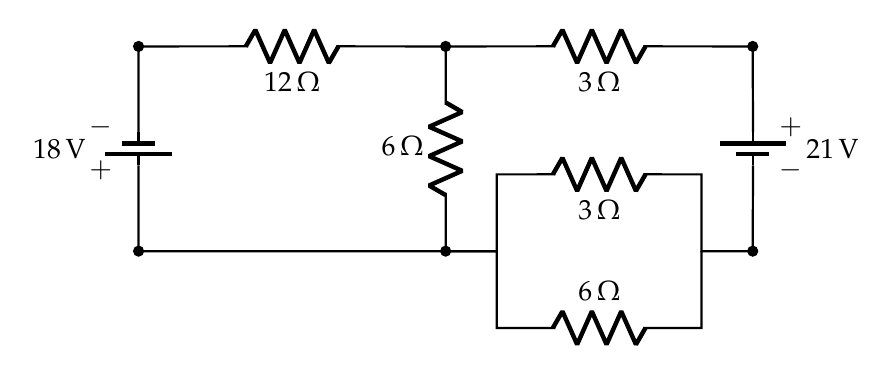
\begin{tikzpicture}[american voltages,scale=1.3]
      \draw[thick](0,0) to[battery1=18<\volt>,*-*] (0,2) to[R,l_=12<\ohm>,-*]
          (3,2) to[R,l_=6<\ohm>,-*] (3,0)--(0,0);
      \draw[thick](3,2) to[R,l_=3<\ohm>,-*] (6,2) to[battery1=21<\volt>,-*]
      (6,0)--(5.5,0)--(5.5,0.75) to[R=3<\ohm>] (3.5,0.75)--(3.5,0)--(3,0);
      \draw[thick](5.5,0)--(5.5,-.75) to[R,l_=6<\ohm>] (3.5,-.75)--(3.5,0)
      --(3,0);
    \end{tikzpicture}
  \end{center}

  \footnotetext[4]{Paul A.\ Tipler, pages 755--756}
\end{frame}


\begin{frame}
  \frametitle{Circuit Analysis \footnotemark}
  \textbf{Example 5:} In the circuit below, the reading of the ammeter is the
  same with both switches open and both closed. Find the resistance $R$.
  \begin{center}
    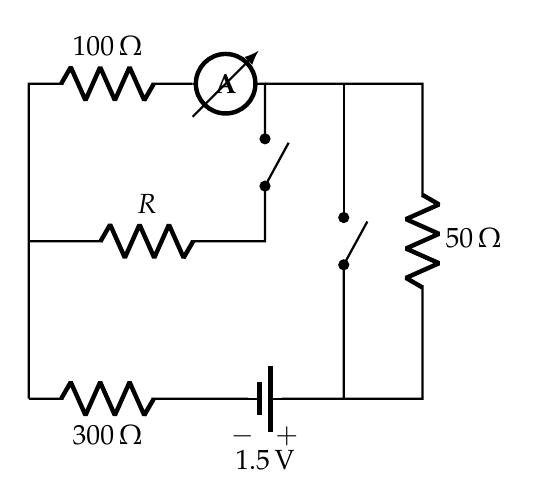
\begin{tikzpicture}[american voltages]
      \draw[thick](0,0)--(0,4) to[R=100<\ohm>](2,4) to[ammeter] (3,4)
      to[short,-*] (3,3.3);
      \draw[thick](3.3,3.25) to[short,-*] (3,2.7)--(3,2) to[R,l_=$R$] (0,2);
      \draw[thick] (3,4)--(5,4) to[R=50<\ohm>] (5,0)--(4,0)
      to[battery1=1.5<\volt>] (2,0) to[R=300<\ohm>] (0,0);
      \draw[thick](4,4) to[short,-*] (4,2.3);
      \draw[thick](4.3,2.25) to[short,-*] (4,1.7)--(4,0);
    \end{tikzpicture}
  \end{center}

  \footnotetext[5]{Paul A.\ Tipler, page 775, problem 30}
\end{frame}


\begin{frame}
  \frametitle{Magnetic Force \footnotemark}
  \begin{columns}
    \column{.6\textwidth}
    \textbf{Example 6:} A point charge $q_1$ is at the point
    $\mb{R}=x\mb{i}+y\mb{j}$ and is moving parallel to the $x$ axis with
    velocity $\mb{v}_1=v_1\mb{i}$. A second point charge $q_2$ is at the origin
    and moving along the $x$ axis with velocity $\mb{v}_2=v_2\mb{i}$. Find the
    magnetic force exerted by each charge on the other.
    
    \column{.4\textwidth}
    \begin{center}
      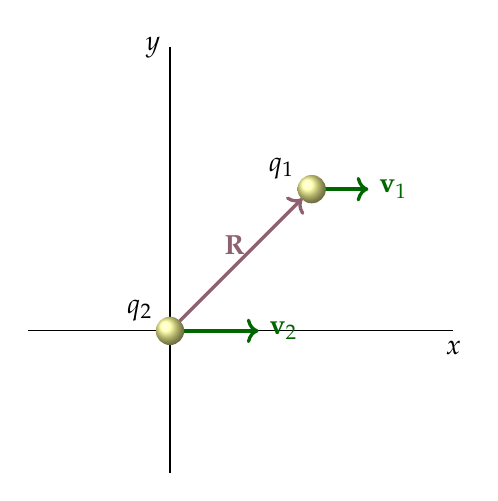
\begin{tikzpicture}[scale=.9]
        \tikzstyle{balloon}=[ball color=yellow!40];
        \draw(-2,0)--(4,0) node[pos=1,below]{$x$};
        \draw(0,-2)--(0,4) node[pos=1,left]{$y$};

        \draw[purple!25!gray,very thick,->,rotate=45](0,0)--(2.64,0)
        node[pos=.65,left] {$\mb{R}$};
        \draw[green!40!black,very thick,->](0,0)--(1.25,0)
        node[pos=1,right] {$\mb{v}_2$};
        \draw[green!40!black,very thick,->](2,2)--(2.8,2)
        node[pos=1,right] {$\mb{v}_1$};
        \shade[balloon] (0,0) circle(0.2) node[above left]{$q_2\;$};
        \shade[balloon] (2,2) circle(0.2) node[above left]{$q_1\;$};
      \end{tikzpicture}
    \end{center}
  \end{columns}

  \footnotetext[6]{Paul A.\ Tipler, pages 814--815}
\end{frame}


\begin{frame}
  \frametitle{Magnetic Field from a Current Loop \footnotemark}
  \textbf{Example 7:} A circular loop of radius \SI{5.0}{\centi\metre} has
  \num{12} turns and lies in the $xy$ plane. It carries a current of
  \SI{4}{\ampere} in the direction such that the magnetic moment of the loop is
  along the $x$ axis. Find the magnetic field on the $x$ axis at 
  \begin{enumerate}
  \item $x=\SI{15}{\centi\metre}$
  \item $x=\SI{3}{\metre}$
  \end{enumerate}

  \footnotetext[7]{Paul A.\ Tipler, pages 817--818}
\end{frame}


\begin{frame}
  \frametitle{Magnetic Field from a Current-Carrying Wire \footnotemark}

  \textbf{Example 8:} An infinitely-long wire carrying current of
  \SI{4.5}{\ampere} is bent as shown in the figure. Find the magnetic field at
  the point $x=\SI{3}{\centi\metre}$, $y=\SI{2}{\centi\metre}$.

  \begin{center}
    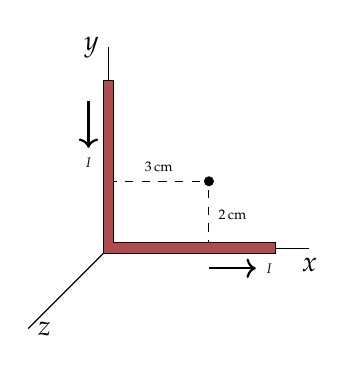
\begin{tikzpicture}[scale=.85]
      \tikzstyle{balloon}=[ball color=yellow!40];
      \draw(0,0)--(3,0) node[pos=1,below]{$x$};
      \draw(0,0)--(0,3) node[pos=1,left]{$y$};
      \draw(0,0)--(-1.2,-1.2) node[pos=1,right]{$z$};
      \draw[dashed](0,1)--(1.5,1) node[midway,above]{\tiny\SI{3}{cm}};
      \draw[dashed](1.5,0)--(1.5,1) node[midway,right]{\tiny\SI{2}{cm}};
      \fill(1.5,1) circle(0.075);
      \draw[fill=red!40!gray](.08,2.5)--(-.08,2.5)--(-.08,-.08)--(2.5,-.08)
      --(2.5,.08)--(.08,.08)--cycle;
      \draw[thick,->](-.3,2.2)--(-.3,1.5) node[pos=1,below]{\tiny $I$};
      \draw[thick,->](1.5,-.3)--(2.2,-.3) node[pos=1,right]{\tiny $I$};
    \end{tikzpicture}
    \end{center}

  \footnotetext[8]{Paul A.\ Tipler, pages 822,825}
\end{frame}

\end{document}

